%% This template was written by Steven Miller and is available here: https://github.com/svmiller/svm-r-markdown-templates/blob/master/svm-latex-ms.tex %%

\documentclass[11pt,]{article}
\usepackage[left=1in,top=1in,right=1in,bottom=1in]{geometry}
\newcommand*{\authorfont}{\fontfamily{phv}\selectfont}
\usepackage[]{mathpazo}


  \usepackage[T1]{fontenc}
  \usepackage[utf8]{inputenc}



\usepackage{abstract}
\renewcommand{\abstractname}{}    % clear the title
\renewcommand{\absnamepos}{empty} % originally center

\renewenvironment{abstract}
 {{%
    \setlength{\leftmargin}{0mm}
    \setlength{\rightmargin}{\leftmargin}%
  }%
  \relax}
 {\endlist}

\makeatletter
\def\@maketitle{%
  \newpage
%  \null
%  \vskip 2em%
%  \begin{center}%
  \let \footnote \thanks
    {\fontsize{18}{20}\selectfont\raggedright  \setlength{\parindent}{0pt} \@title \par}%
}
%\fi
\makeatother




\setcounter{secnumdepth}{0}


\usepackage{graphicx}
% We will generate all images so they have a width \maxwidth. This means
% that they will get their normal width if they fit onto the page, but
% are scaled down if they would overflow the margins.
\makeatletter
\def\maxwidth{\ifdim\Gin@nat@width>\linewidth\linewidth
\else\Gin@nat@width\fi}
\makeatother
\let\Oldincludegraphics\includegraphics
\renewcommand{\includegraphics}[1]{\Oldincludegraphics[width=\maxwidth]{#1}}

\title{Thesis Title: Thesis Subtitle  }



\author{\Large Victoria Wickham\vspace{0.05in} \newline\normalsize\emph{Major and Department}   \and \Large Dr.~Megan L. Larsen\vspace{0.05in} \newline\normalsize\emph{Water Sciences Laboratory, University of Nebraska-Lincoln}  }


\date{}

\usepackage{titlesec}

\titleformat*{\section}{\normalsize\bfseries}
\titleformat*{\subsection}{\normalsize\itshape}
\titleformat*{\subsubsection}{\normalsize\itshape}
\titleformat*{\paragraph}{\normalsize\itshape}
\titleformat*{\subparagraph}{\normalsize\itshape}


\usepackage{natbib}
\bibliographystyle{apsr}
\usepackage[strings]{underscore} % protect underscores in most circumstances



\newtheorem{hypothesis}{Hypothesis}
\usepackage{setspace}

\makeatletter
\@ifpackageloaded{hyperref}{}{%
\ifxetex
  \PassOptionsToPackage{hyphens}{url}\usepackage[setpagesize=false, % page size defined by xetex
              unicode=false, % unicode breaks when used with xetex
              xetex]{hyperref}
\else
  \PassOptionsToPackage{hyphens}{url}\usepackage[unicode=true]{hyperref}
\fi
}

\@ifpackageloaded{color}{
    \PassOptionsToPackage{usenames,dvipsnames}{color}
}{%
    \usepackage[usenames,dvipsnames]{color}
}
\makeatother
\hypersetup{breaklinks=true,
            bookmarks=true,
            pdfauthor={Victoria Wickham (Major and Department) and Dr.~Megan L. Larsen (Water Sciences Laboratory, University of Nebraska-Lincoln)},
             pdfkeywords = {harmful algal blooms, frequency, intensity, Nebraska lakes},  
            pdftitle={Thesis Title: Thesis Subtitle},
            colorlinks=true,
            citecolor=blue,
            urlcolor=blue,
            linkcolor=magenta,
            pdfborder={0 0 0}}
\urlstyle{same}  % don't use monospace font for urls



% add tightlist ----------
\providecommand{\tightlist}{%
\setlength{\itemsep}{0pt}\setlength{\parskip}{0pt}}

\begin{document}
	
% \pagenumbering{arabic}% resets `page` counter to 1 
%
% \maketitle

{% \usefont{T1}{pnc}{m}{n}
\setlength{\parindent}{0pt}
\thispagestyle{plain}
{\fontsize{18}{20}\selectfont\raggedright 
\maketitle  % title \par  

}

{
   \vskip 13.5pt\relax \normalsize\fontsize{11}{12} 
\textbf{\authorfont Victoria Wickham} \hskip 15pt \emph{\small Major and Department}   \par \textbf{\authorfont Dr.~Megan L. Larsen} \hskip 15pt \emph{\small Water Sciences Laboratory, University of Nebraska-Lincoln}   

}

}







\begin{abstract}

    \hbox{\vrule height .2pt width 39.14pc}

    \vskip 8.5pt % \small 

\noindent Some really good stuff here with 1-2 sentences from the INTRO, RESULTS,
and CONCLUSIONS. This section should be no longer than 300 words.


\vskip 8.5pt \noindent \emph{Keywords}: harmful algal blooms, frequency, intensity, Nebraska lakes \par

    \hbox{\vrule height .2pt width 39.14pc}



\end{abstract}


\vskip 6.5pt

\noindent   \clearpage
\tableofcontents  \newpage
\listoftables  \newpage
\listoffigures  \newpage

\section{Introduction}\label{introduction}

We can create citations like this:

\begin{itemize}
\tightlist
\item
  To suppress the author's name: \citet{smith2017a} had some really
  great things to say.
\item
  Or to include the full citation: One of his other articles completely
  contradicted the first \citep{smith2017b}
\end{itemize}

\section{Methods}\label{methods}

\subsection{Study system and data
collection}\label{study-system-and-data-collection}

Describe the lakes and hwo the data was collected

\subsection{Data sources}\label{data-sources}

\subsection{Analyses and calculations}\label{analyses-and-calculations}

\subsubsection{Frequency}\label{frequency}

\subsubsection{Intensity}\label{intensity}

\subsection{Statistics}\label{statistics}

\section{Results}\label{results}

\subsection{Summarize result 1 in a single
sentence.}\label{summarize-result-1-in-a-single-sentence.}

The frequency of algal blooms across the state of Nebraska increased by
X\% between 2005 - 2015 (\autoref{fig1}).

\begin{figure}[htbp]
\centering
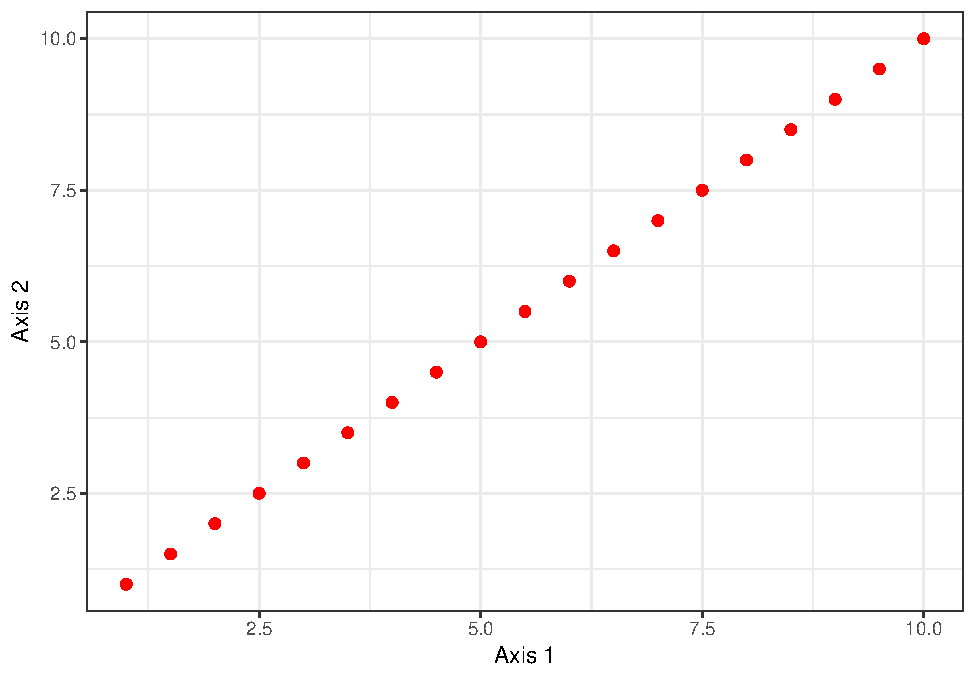
\includegraphics{wickham-thesis_files/figure-latex/fig1-1.pdf}
\caption{A descriptive title about the frequency. \label{fig1}}
\end{figure}

\subsection{Summarize result 2 in a single
sentence.}\label{summarize-result-2-in-a-single-sentence.}

Some great text about this!

\section{Conclusions}\label{conclusions}
\newpage
\singlespacing 
\renewcommand\refname{References}
\bibliography{C:/Users/meglarse/Desktop/wickham-thesis/doc-setup/wickham-thesis-bib}
\end{document}